\documentclass[10pt]{beamer}
\usetheme[progressbar=frametitle]{metropolis}
\usepackage{appendixnumberbeamer}
\usepackage{booktabs}
\usepackage{xspace}
\usepackage[backend=biber,style=alphabetic]{biblatex}

\addbibresource{references.bib}
\ExecuteBibliographyOptions{isbn=false,url=false,doi=true,eprint=false}
\DeclareSourcemap{
  \maps[datatype=bibtex, overwrite]{
    \map{
      \step[fieldset=editor, null]
      \step[fieldset=booktitle, null]
      \step[fieldset=series, null]
      \step[fieldset=pages, null]
      \step[fieldset=address, null]
      \step[fieldset=journal, null]
      \step[fieldset=publisher, null]
      \step[fieldset=volume, null]
      \step[fieldset=number, null]
      \step[fieldset=note, null]
    }
  }
}

\def\do#1{
  \DeclareBibliographyDriver{#1}{%
    \usebibmacro{bibindex}%
    \usebibmacro{begentry}%
    \usebibmacro{author/editor+others/translator+others}%
    \setunit{\labelnamepunct}\newblock
    \usebibmacro{title}%
    \newunit\newblock
    \usebibmacro{date}%
    \newunit\newblock
    \iftoggle{bbx:doi}
      {\printfield{doi}}
      {}%
    \setunit{\bibpagerefpunct}\newblock
    \usebibmacro{pageref}%
    \newunit\newblock
    \usebibmacro{finentry}}}
\makeatother


\newcommand{\PresQ}[0]{\textsc{PresQ}\xspace}
\newcommand{\eqdist}{\stackrel{d}{=}}

% 2. El acto consistirá en la exposición oral por el doctorando del trabajo de
% investigación elaborado ante los miembros del tribunal, refiriéndose
% principalmente a la labor realizada, la metodología, el contenido y las conclusiones,
% haciendo especial mención de sus aportaciones originales.

% Evaluación
% i. Justificación del carácter innovador del tema de estudio.
% ii. Adecuación de la metodología utilizada o propuesta de alternativas
% iii. Grado de claridad en la exposición de los resultados obtenidos y análisis de los mismos.
% iv. Observación de la correcta elección y citación de la bibliografía.
% v. Análisis crítico de las conclusiones de estudio.

% Creo que las mismas secciones que la tesis, pero tampoco es plan de ser redundante?

\title{Navigating Diverse Datasets\\
in the Face of Uncertainty}
\subtitle{}
% \date{\today}
\date{}
\author{Alejandro Álvarez Ayllón}
\institute{Programa Oficial de Doctorado en Ingeniería Informática de la Universidad de Cádiz}
\titlegraphic{\hfill
\includegraphics[height=1.5cm]{uca-logo.pdf}}

\begin{document}

\maketitle

\section{Introduction}

\begin{frame}{Motivation}
\begin{enumerate}
    \item Data exploration represents the fourth paradigm of scientific exploration, alongside experimental, theoretical, and computer-simulation paradigms.
    \item Data exploration is a vital component of the data-intensive scientific process.
    \item Researchers must curate, understand, and extract information from data-sets.
    \item To extract knowledge, first they need to identify patterns: \alert{data mining}.
\end{enumerate}
\end{frame}

\begin{frame}{}
\begin{figure}
    \centering
    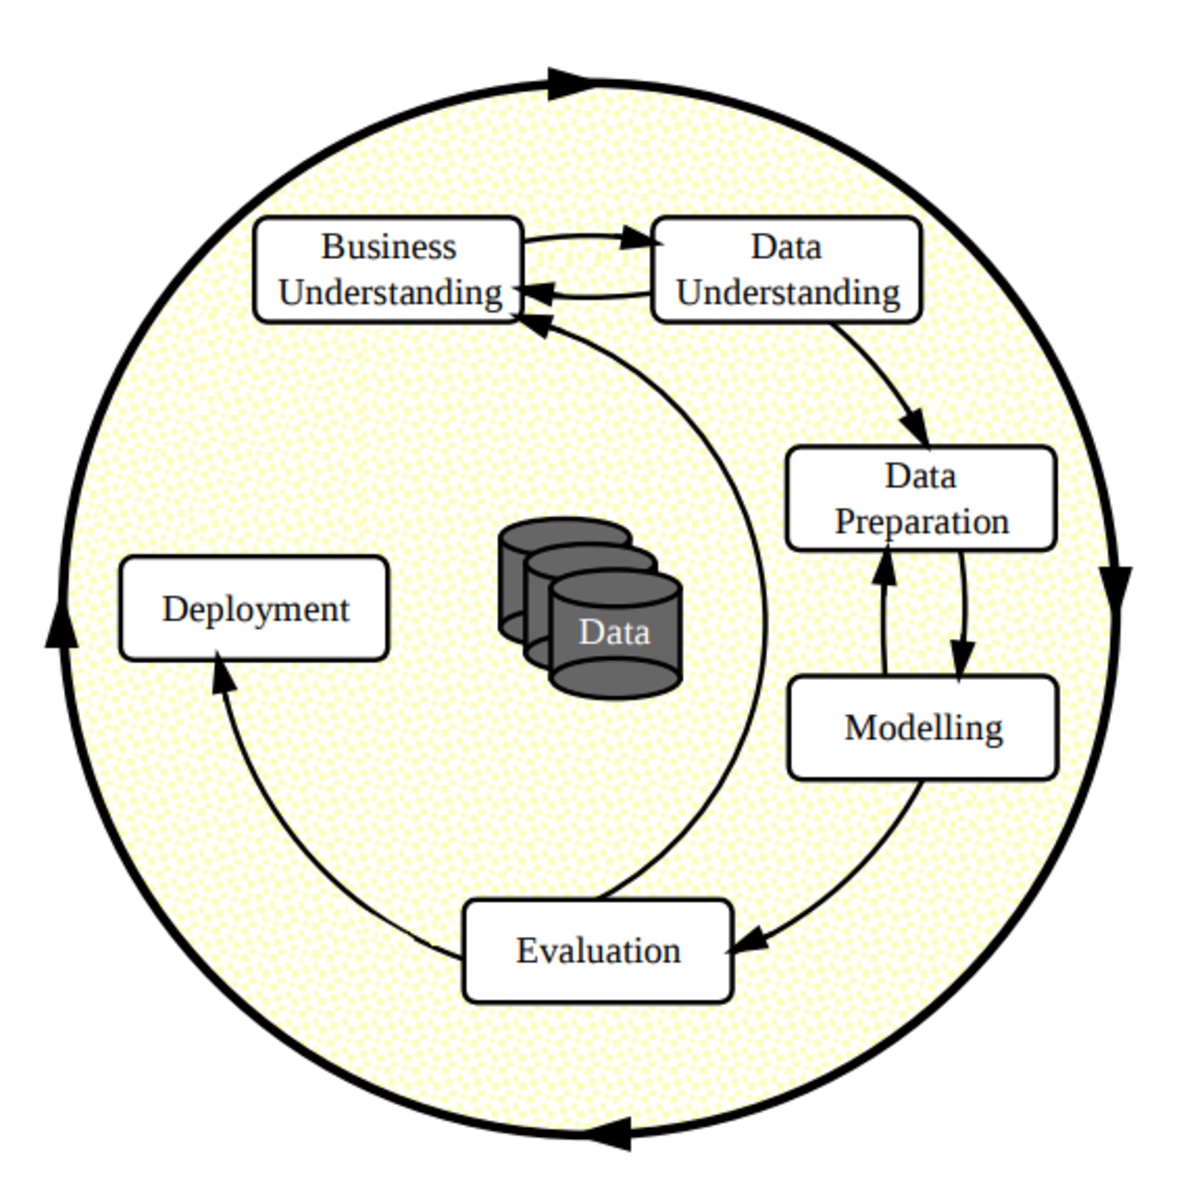
\includegraphics[height=0.8\textheight]{crisp-dm.pdf}
    \caption{CRoss Industry Standard Process for Data Mining}
\end{figure}
\end{frame}

\begin{frame}{Our Focus: Data Understanding}

The \alert{familiarization with the data}. The user interactively explores the
data, gaining insight, and generating new hypotheses.

During this stage, the data may be stored in unprocessed files, with an
inconsistent or poorly documented schema.

\end{frame}

\begin{frame}{Objectives}
\begin{alertblock}{Main Objective}
    \smallskip
    To assist data scientists during the exploration of unprocessed, numerical, raw data distributed across multiple
    files based solely on its intrinsic distribution.
\end{alertblock}

\begin{block}{Sub-objectives}
    \begin{enumerate}
        \item Find existing techniques that help users to explore the data in-situ.
        \item Identify gaps in the coverage of the existing techniques.
        \item Design new algorithms tailored to numerical and uncertain data.
    \end{enumerate}
\end{block}
\end{frame}



\section{Methodology}

\begin{frame}{Framework}
\begin{block}{\alert{Researching Information Systems and Computing}~\cite{Oates2006}}

\begin{description}
    \item[Purpose] The stated objective.
    \item[Products] Analysis of the state-of-the-art, and a two new algorithms.
    \item[Process] See next slide.
    \item[Participants] Researcher, supervisor, reviewers.
    \item[Paradigm] \emph{Pragmatism}~\cite{Shull2008}.
    \item[Presentation] Papers, posters, published software, the current dissertation, etc.
\end{description}

\end{block}
\end{frame}

\begin{frame}{Process}

\begin{alertblock}{Literature Review}
    \emph{Systematic Literature Mapping}~\cite{Petersen2007}, a process for the exploration of
    the situation of a wide research area with a high level of granularity.
\end{alertblock}

\begin{alertblock}{Strategy}
    \emph{Engineering Design}~\cite{Dym2012}, the systematic, intelligent generation and evaluation
    of specifications for artifacts whose form and function achieve stated objectives and satisfy specified
    constraints.
\end{alertblock}

\begin{alertblock}{Data Generation Methods}
Observations (experiments), to evaluate preliminary products.
\end{alertblock}

\begin{alertblock}{Data Analysis}
    Quantitative
\end{alertblock}

\end{frame}

\section{State of the Art}

\begin{frame}{Systematic Literature Mapping}
\begin{figure}
    \begin{alertblock}{Questions}
        \begin{itemize}
            \item RQ1. How has the research area evolved?
            \item RQ2. What is the maturity level of the research area?
            \item RQ3. How far are we from an interactive tool that provides access to raw data files stores in distributed storage?
        \end{itemize}
    \end{alertblock}
    \begin{block}{Search strategy}
        \begin{itemize}
            \item Digital Libraries (ACM, Elsevier, Springer, IEEE)
            \item Forward Snowballing
        \end{itemize}
        Two searches: 2017 and 2022.
    \end{block}
\end{figure}
\end{frame}

\begin{frame}{Classification}
  \begin{columns}[t, totalwidth=1.02\textwidth]
    \metroset{block=fill}
    \begin{column}{0.45\linewidth}
        \begin{block}{Category~\cite{Idreos2015}}
            Three main layers:
            \begin{itemize}
                \item Database Layer
                \item Middleware
                \item User Interaction
            \end{itemize}
        \end{block}
    \end{column}
    \begin{column}{0.45\linewidth}
        \begin{block}{Research type~\cite{Wieringa2006}}
            \begin{itemize}
                \item Validation Research
                \item Proposal of Solution
                \item Evaluation Research
                \item Philosophical Paper
                \item Opinion Paper
            \end{itemize}
        \end{block}
    \end{column}
    \end{columns}
\end{frame}

\begin{frame}{}
\begin{figure}
    \centering
    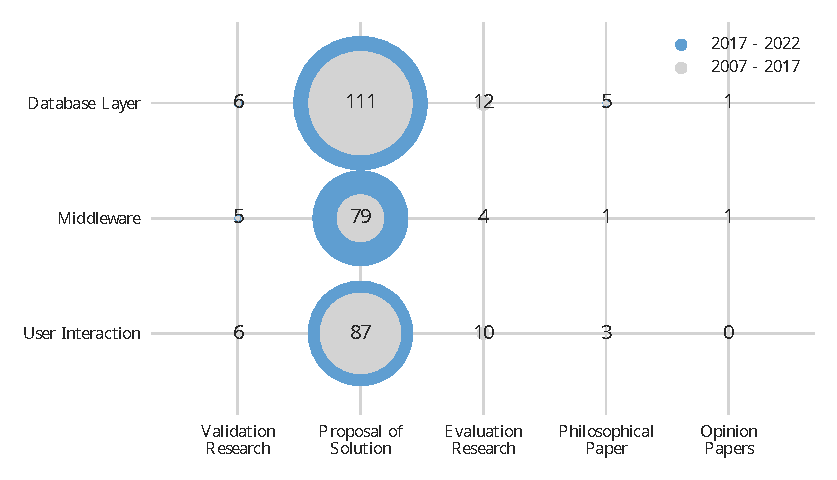
\includegraphics[width=\textwidth]{layer_vs_type.pdf}
    \caption{Layer vs Study research type.}
\end{figure}
\end{frame}

\begin{frame}{Conclusions}
    \begin{block}{RQ1. How has the research area evolved?}
        \smallskip
        All three layers are well studies, but the middleware layer is becoming a more popular target.
    \end{block}
    \begin{block}{RQ2. What is the maturity level of the research area?}
        \smallskip
        The vast majority of studies are \emph{Proposal of Solutions}. There is very little follow-up of implementations in practice.
    \end{block}
\end{frame}

\begin{frame}{Conclusions}
    \begin{block}{RQ3. How far are we from a tool that solves our three requirements?}
        \begin{figure}
            \centering
            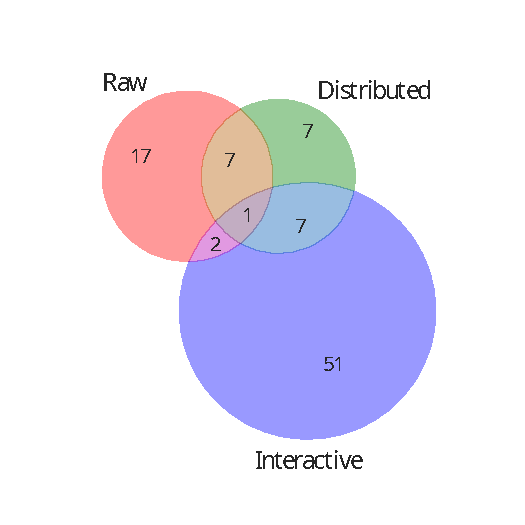
\includegraphics[width=0.6\textwidth]{venn.pdf}
        \end{figure}
    \end{block}
\end{frame}

\begin{frame}{Insights}
    \begin{block}{}
        Most solutions treat files as separate, independent, relations~\cite{Silva2016}. They offer
        little to no assistance in finding relations that \textit{overlap}.
    \end{block}
    \begin{block}{}
        One exception is \textsc{Kayak}~\cite{maccioni_crossing_2017}.
        \begin{itemize}
            \item Integrates \textsc{Metanome}~\cite{papenbrock2015data}.
            \item Based on \emph{Inclusion Dependencies} (IND), which assume discrete data types.
        \end{itemize}
    \end{block}
    \begin{block}{}
        ``Identifying Relationships between Scientific Datasets''~\cite{alawini2016} is close, but does not
        consider multidimensional attributes (i.e. photometry in astronomy).
    \end{block}
    \alert{\textbf{Can we generalize IND to uncertain, multidimensional sets of attributes?}}
\end{frame}

\section{\PresQ}

\begin{frame}{}
\begin{figure}
    \centering
    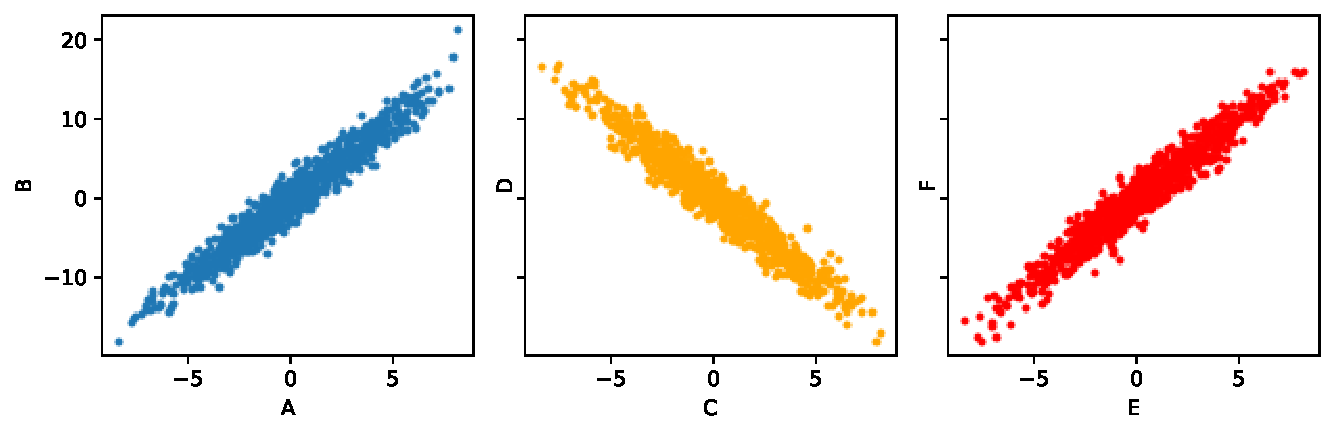
\includegraphics[width=\textwidth]{no2ind.pdf}
    \caption{Example of a 2D distribution where the pairwise matching is not enough.}
\end{figure}
\end{frame}

\subsection{Background}

\begin{frame}{Inclusion Dependencies}
\end{frame}

\begin{frame}{Example of Lattice}
\begin{figure}
    \centering
    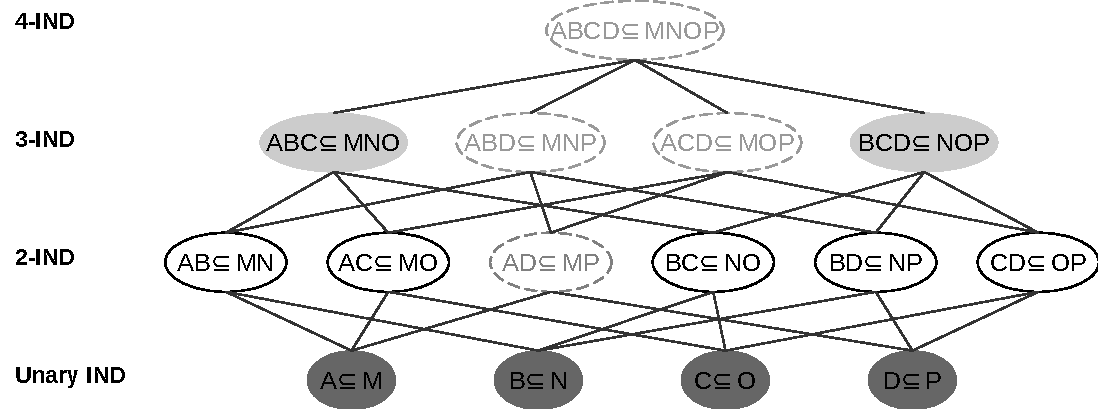
\includegraphics[width=\textwidth]{lattice.pdf}
    \caption{
    Example structure of the search space as a lattice for an initial set
    of 4 unary Inclusion Dependencies.
    }
\end{figure}
\end{frame}

\begin{frame}{Bottom-Up Search}
    \begin{alertblock}{Complexity}
    If we have an n-EDD between two datasets, and traverse the lattice bottom-up, we need
    to test...
    
    \begin{equation*}
        \sum_{k=0}^{n}{\binom{n}{k}} = \sum_{k=0}^{n} \frac{n!}{n!(n - k)!}
    \end{equation*}
    
    possible combinations of attributes.
    \end{alertblock}
\end{frame}

\begin{frame}{Complexity}

    It turns out that finding INDs/EDDs is one of the hardest computer science
    problems~\cite{Blsius2017}.
    
    \begin{itemize}
        \item It is \textbf{NP-complete}.
        \item The \textbf{number of solutions} can be \textbf{exponential} in the input size.
        \item It is \textbf{non approximable} (NP-complete even if we accept an error margin).
    \end{itemize}
    
    \bigskip
    
    However, the run-time can be reasonable if we are optimistic: i.e. if we assume
    $n$ 1EDD are derived from a single $n$EDD, we only need one test!: top-down traversal.
    
    \bigskip
    
    But we risk being too optimistic\ldots
\end{frame}

\subsection{Clique Finding}
\begin{frame}{Clique Finding}
    The problem can be mapped to finding cliques on hypergraphs (\textsc{Find}~\cite{koeller2003discovery}):
    
    \begin{enumerate}
        \item Pairwise matches (1EDD) are mapped to \textbf{nodes}.
        \item $k$-combinations of 1EDD are mapped to \textbf{$k$-edges}.
        \item Cliques of size $n$ \emph{may} correspond to $n$EDD.
        \item If they are not, we \emph{break} these cliques into a set of $k+1$ edges and
            validate them.
    \end{enumerate}
\end{frame}

\begin{frame}{Clique Finding}
    \begin{exampleblock}{Example}
        \begin{columns}
        \begin{column}{.7\textwidth}
        \begin{enumerate}
            \item $A \eqdist M, B \eqdist N, C \eqdist O, D \eqdist P$
            \item All 6 possible 2-EDD are true
            \item Clique with 4 nodes $ABCD \eqdist MNOP$
            \item If false, we break it into
                \begin{enumerate}
                    \item $ABC \eqdist MNO$
                    \item $BCD \eqdist NOP$
                    \item $ACD \eqdist MOP$
                    \item \ldots
                \end{enumerate}
        \end{enumerate}
        \end{column}
        \begin{column}{.3\textwidth}
            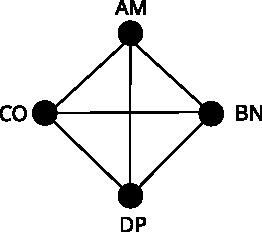
\includegraphics[width=\linewidth]{4clique}
        \end{column}
        \end{columns}
    \end{exampleblock}
    
    \pause
    
    \begin{alertblock}{}
    But we are using statistical tests.
    
    \begin{itemize}
        \item We may falsely refuse an EDD (type I error)
        \item Or falsely accept it (type II error).
    \end{itemize}
    \end{alertblock}
\end{frame}


\subsection{Quasi-Clique Finding}
\begin{frame}{Quasi-Clique Finding}
    Is a clique with missing edges, which can be limited as a ratio of the total (1)
    or as a ratio of the degree of a node (2).

    \metroset{block=fill}
    \begin{alertblock}{Definition}
    Given a k-uniform hypergraph $(V,E)$, and two parameters $\lambda, \gamma \in [0,1]$,
    the sub-graph $H'=(V',E')$ induced by a subset $V' \subseteq V$ is a
    $(\lambda-\gamma)$ quasi-clique iff:
    
    \begin{equation}
        |E'| \ge \gamma \cdot \binom{|V'|}{k}
        \label{eq:edge_hyperclique}
    \end{equation}
    
    \begin{equation}
        \forall v \in V': deg_{V'}(v) \ge \lambda \cdot \binom{|V'| - 1}{k - 1}
        \label{eq:deg_hyperclique}
    \end{equation}

    Where $deg_{V'}(v)$ represents the degree of $v$, and $E'$ is a subset of $E$ such that
    $\forall e \in E' : e \subseteq V'$
    \end{alertblock}
    
    We can approximate $\gamma \approx 1 - \alpha$. How do we bound $\lambda$ ?
\end{frame}

\begin{frame}{Quasi-Clique Finding}
    \begin{block}{}
    There is no reason to think that any particular subset of the edges
    has a higher probability of having missing members. If a given node has an
    unexpectedly low degree, it is most likely connected by spurious edges.
    
    The degree of the nodes should follow a hypergeometric distribution:
    \end{block}
    \centering
    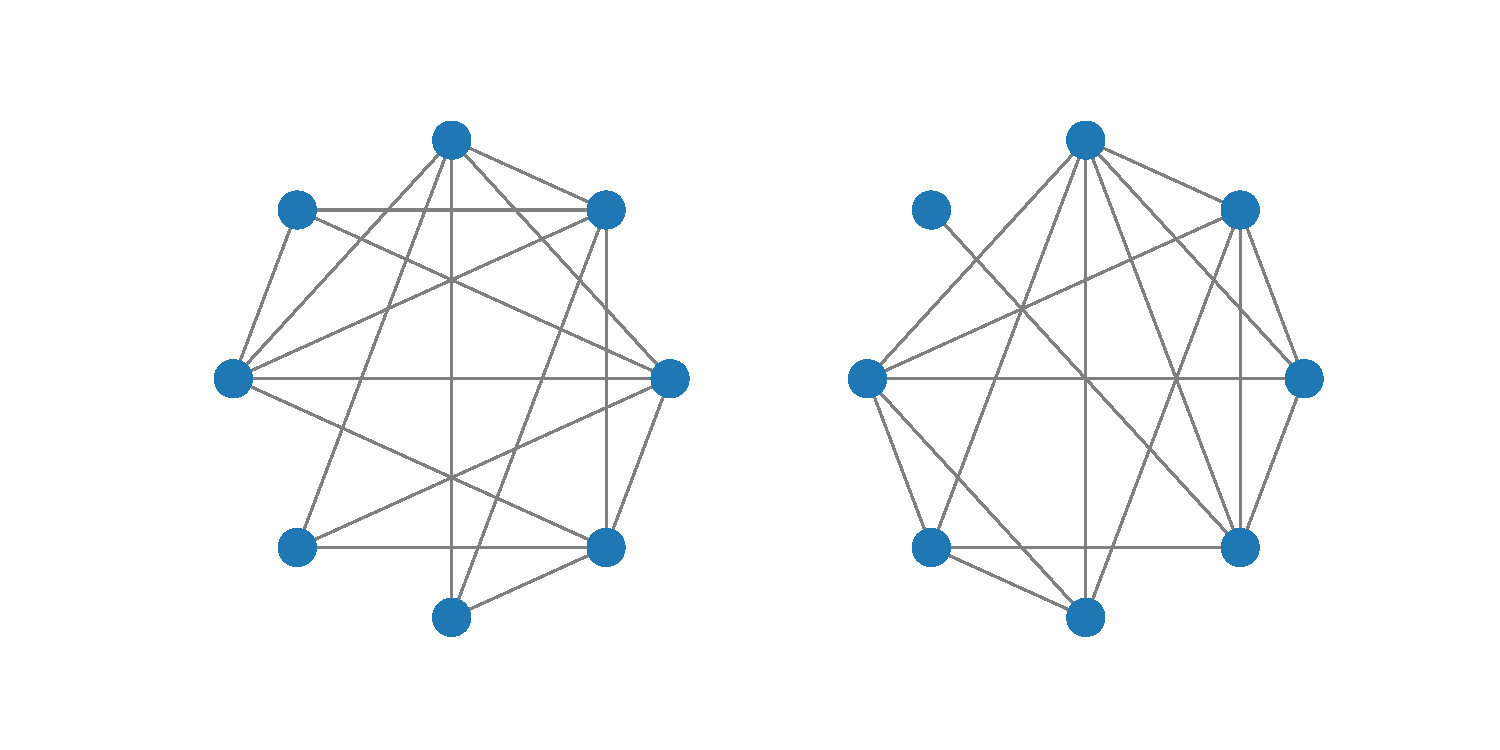
\includegraphics[width=0.7\linewidth]{quasicliques}
\end{frame}

\begin{frame}{\PresQ}

    \begin{block}{}
    \PresQ~\cite{AlvarezAyllonPresQ2022} is an algorithm for finding quasi-cliques on uniform
    $k$-hypergraphs.
    
    \begin{enumerate}
        \item Finds ``seeds'' using a modified version of \textsc{Hyperclique}~\cite{koeller2003discovery}.
        \item Grows the ``seeds'' following a tree-shaped, depth-first
        traversal~\cite{uno_efficient_2010}.
    \end{enumerate}
    \end{block}
    
    \begin{alertblock}{Complexity}
        The number of maximal cliques is bound in general by $\Omega(a^{|V|/b})$,
        where $a, b$ are two constants that depend on the rank of the hypergraph~\cite{Tomescu1981}.
        
        The worst-case is always going to be exponential for this problem.
    \end{alertblock}
\end{frame}

\subsection{Algorithm}

\begin{frame}{Quasi-Cliques}
\end{frame}

\begin{frame}{Finding seeds}
\end{frame}

\begin{frame}{Growing quasi-cliques}
\end{frame}

\begin{frame}{Validation}
\end{frame}

\subsection{Experiments}

\begin{frame}{Experimental Setup}
    
\end{frame}

\begin{frame}{}
\begin{figure}
    \centering
    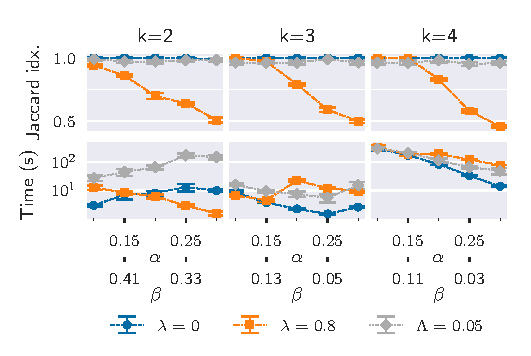
\includegraphics[width=\textwidth]{quasi_corr_20.eps}
    \caption{
    Recovery ratio and run-times for cliques of size 20 on uniform $(2,3,4)$-hypergraphs.
    }
\end{figure}
\end{frame}

\begin{frame}{}
\begin{figure}
    \centering
    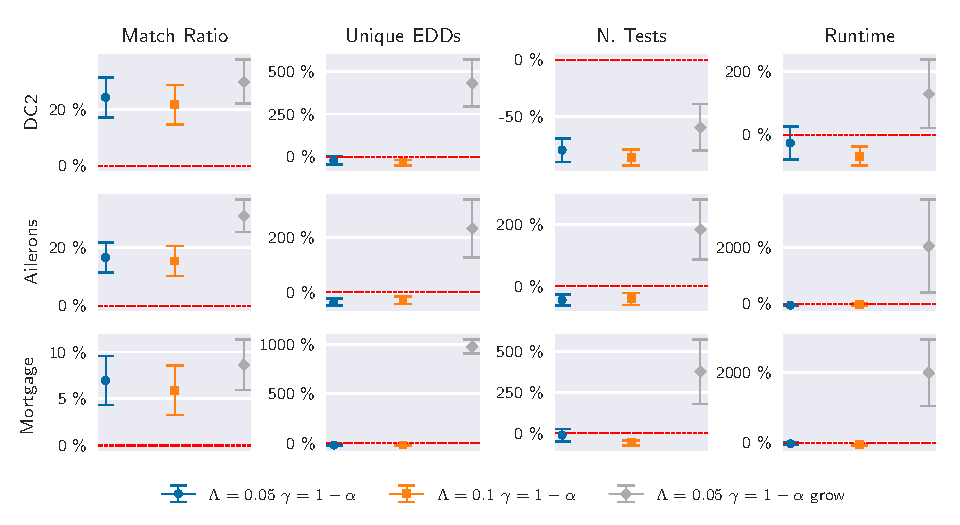
\includegraphics[width=\textwidth]{all.eps}
    \caption{$95\%$ confidence intervals for the percent difference
    between \textsc{Find} and \PresQ.}
\end{figure}
\end{frame}

\begin{frame}{}
\begin{figure}
    \centering
    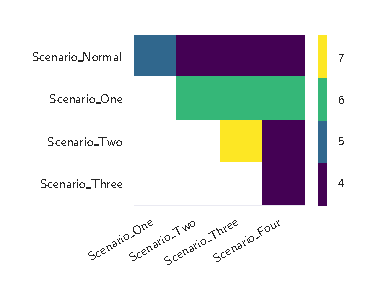
\includegraphics{afds.eps}
    \caption{Pairwise max arity found on the AFDS dataset for each pair of scenarios.}
\end{figure}
\end{frame}

\section{Two-Sample Test Based on Self-Organizing Maps}

\subsection{Background}

\begin{frame}{Classifier 2-Sample Tests}
\end{frame}

\begin{frame}{Self-Organizing Maps}
\end{frame}

\subsection{Algorithm}

\begin{frame}{SOM 2-Sample Test}
\end{frame}

\subsection{Experiments}

\begin{frame}{Experimental Setup}
    
\end{frame}

\begin{frame}{}
\begin{figure}
    \centering
    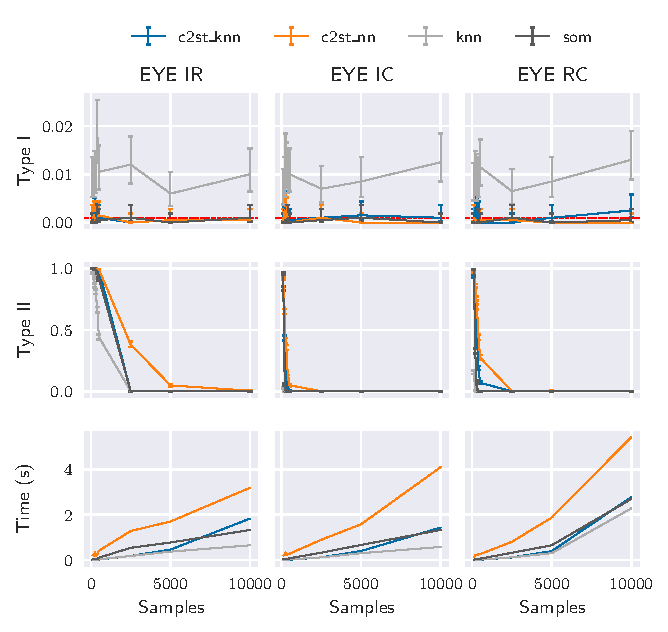
\includegraphics[height=\textheight]{eye.pdf}
\end{figure}
\end{frame}

\begin{frame}{}
\begin{figure}
    \centering
    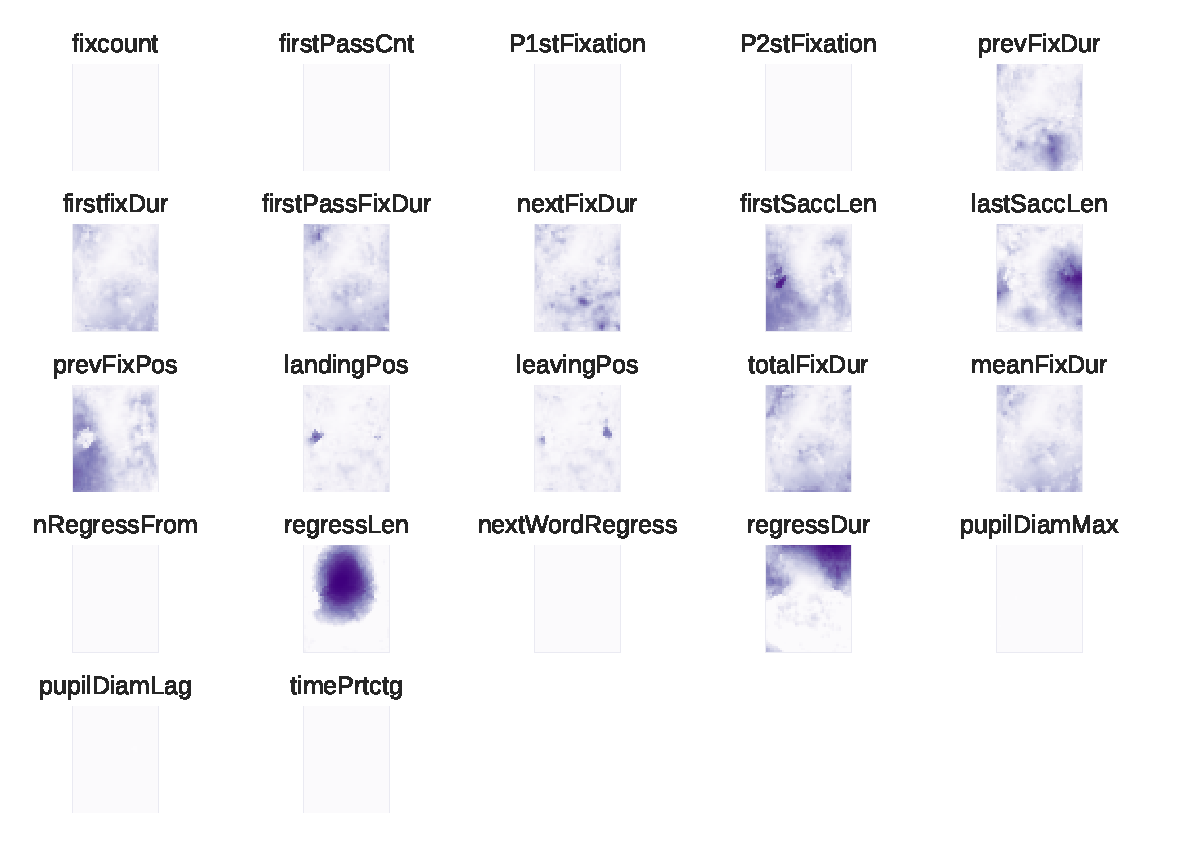
\includegraphics[width=\textwidth]{eye_features.eps}
\end{figure}
\end{frame}

\begin{frame}{}
\begin{figure}
    \centering
    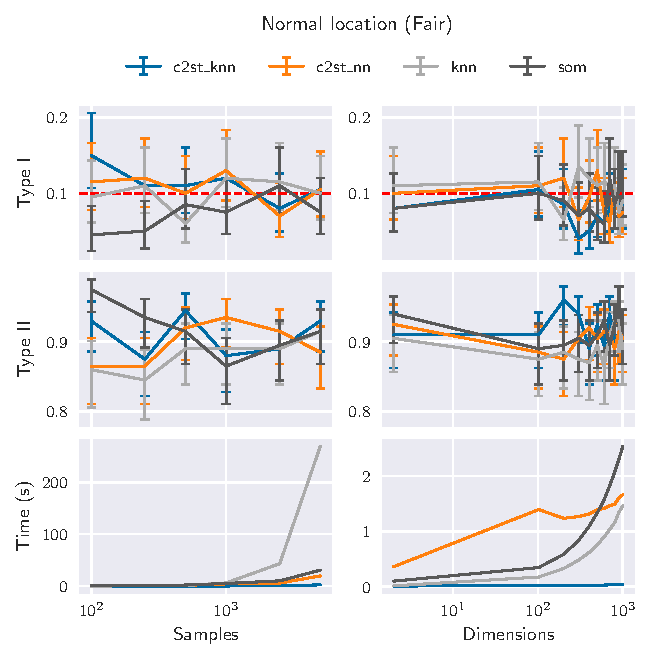
\includegraphics[height=\textheight]{normal_location_fair.pdf}
\end{figure}
\end{frame}

\section{Discussion}

\begin{frame}{\PresQ}
\end{frame}

\begin{frame}{Two-Sample Test Based on SOM}
\end{frame}

\begin{frame}{Threats to Validity}
\end{frame}

\section{Conclusions}

\begin{frame}{Contributions}
\end{frame}

\begin{frame}{Future Work}
\end{frame}



\begin{frame}[allowframebreaks]{Bibliography}
\printbibliography[]
\end{frame}

\appendix

{\setbeamercolor{palette primary}{fg=white, bg=black}
\begin{frame}[standout]
  Backup slides
\end{frame}
}

\begin{frame}{}
\begin{figure}
    \centering
    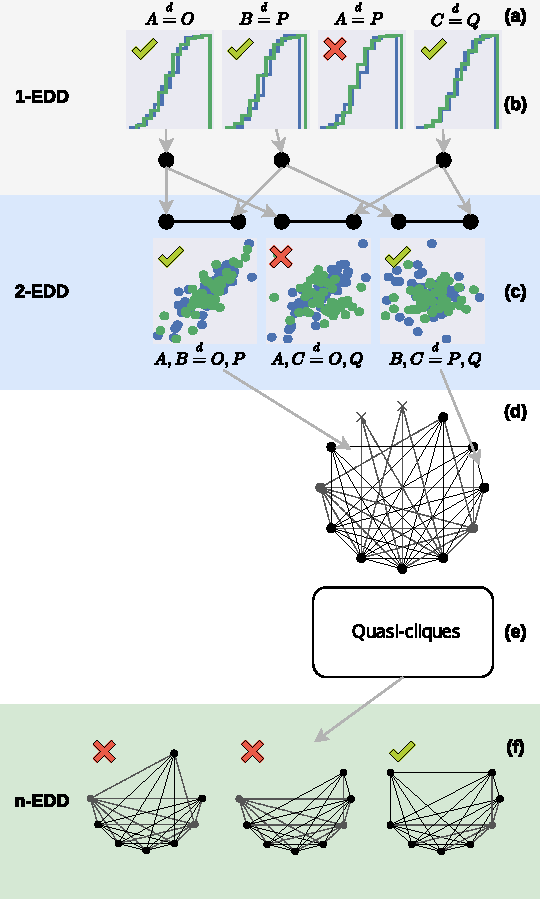
\includegraphics[height=\textheight]{pipeline.pdf}
\end{figure}
\end{frame}

\begin{frame}{}
\begin{figure}
    \centering
    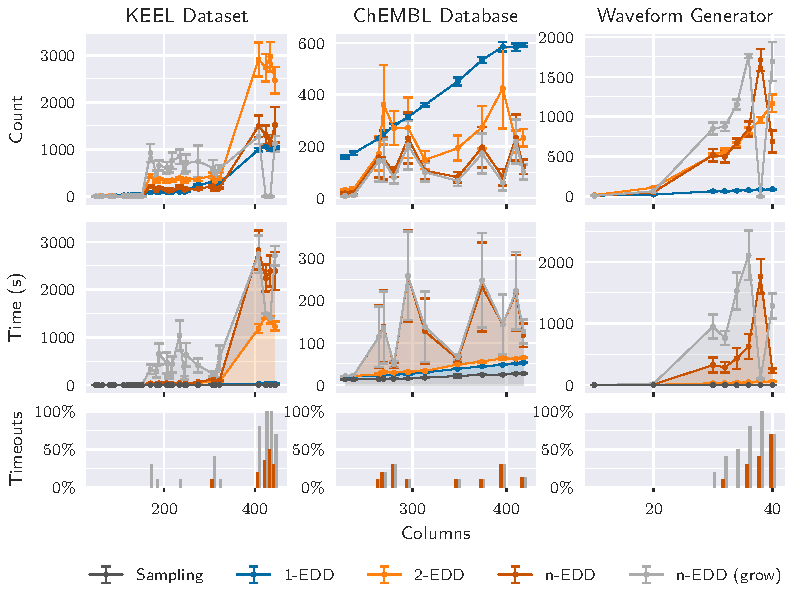
\includegraphics[width=\textwidth]{scalability.pdf}
\end{figure}
\end{frame}

\begin{frame}{}
\begin{figure}
    \centering
    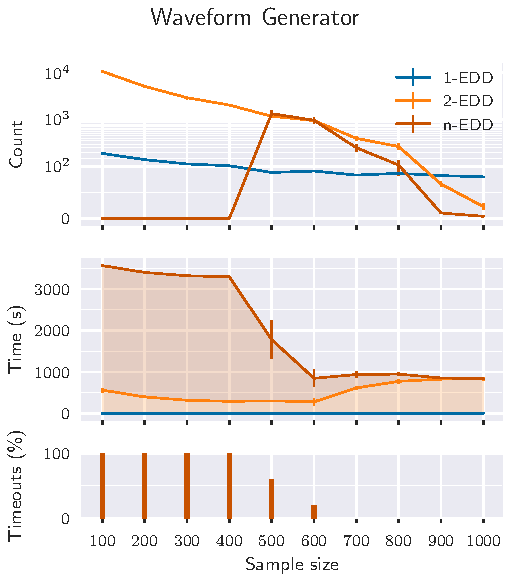
\includegraphics[height=\textheight]{scalability_sample_wave.pdf}
\end{figure}
\end{frame}

\begin{frame}{}
\begin{figure}
    \centering
    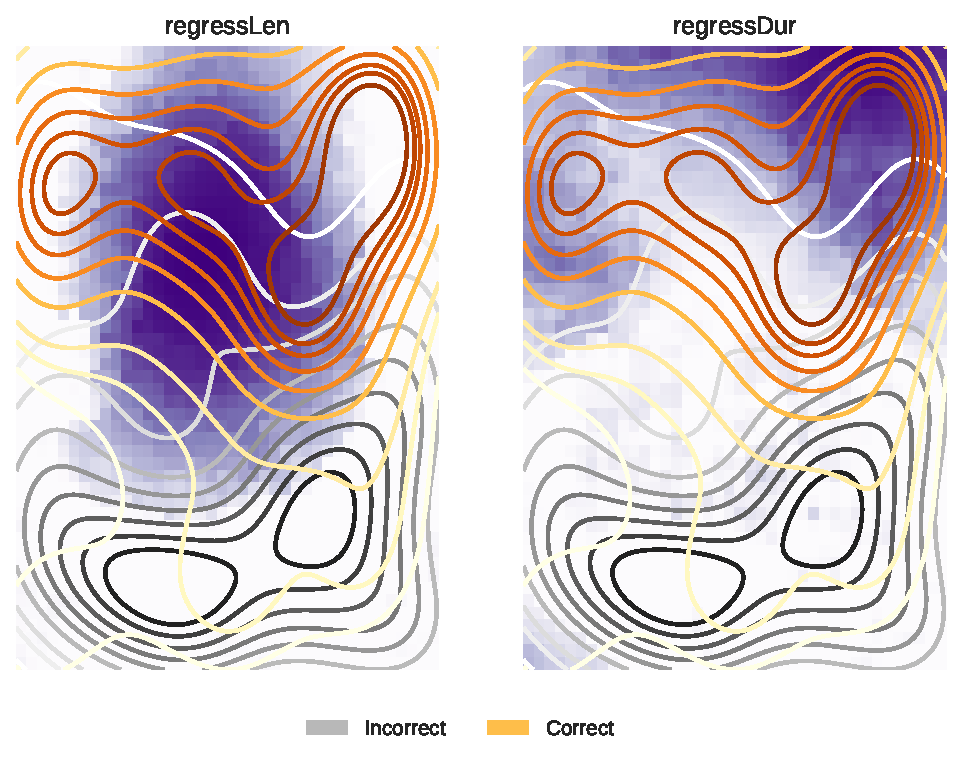
\includegraphics[height=\textheight]{eye_regress-eps-converted-to.pdf}
\end{figure}
\end{frame}

\end{document}
